In order to keep a good structure on the program and a logical separation of functionalities, several data structures have been created.

\begin{figure}[htb]
	\centering
	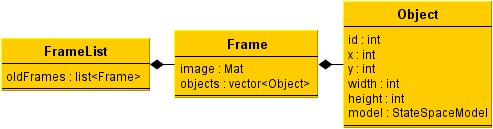
\includegraphics[width=150mm]{images/data_structures_uml.png}
	\caption{\textit{UML diagram of the main data structures. A video is represented by a FrameList, containing each Frame of the video. Each such Frame contains the detected objects in that image and each object contains spatial information, a unique id and a StateSpaceModel used for the Kalman filter prediction}}
	\label{fig:UML_fig} %Skapar referens till figuren
\end{figure}

%\subsubsection{ProbabilityMap}
%DErpa derpa derpa derpa. DErpa derpa derpa derpa.DErpa derpa derpa derpa.DErpa derpa derpa derpa.DErpa derpa derpa derpa.DErpa derpa derpa derpa.DErpa derpa derpa derpa.
%DErpa derpa derpa derpa.DErpa derpa derpa derpa.DErpa derpa derpa derpa.DErpa derpa derpa derpa.DErpa derpa derpa derpa.DErpa derpa derpa derpa.DErpa derpa derpa derpa.
%DErpa derpa derpa derpa. See code in appendix \ref{sec:ProbMap_code}. \cite{CVBook} % reference to bilbliography

\subsubsection{Object}
The \emph{Object} class represents a moving object in the scene. The information stored about the objects is ID, position, velocity, and bounding box. This information is what is processed in the object identification and prediction models. 

\subsubsection{Frame}
The \emph{Frame} class contains the current image as well as the probability map. Both if these are stored as \emph{cv::Mat}. The image is used for creation of the probability map as well as drawing the bounding boxes. From the probability map The foreground processing module finds and creates Objects that are stored in a vector. To draw the objects and their bounding boxes in the image, the function \emph{DrawObject} is called with the appropriate color. \ref{fig:UML_fig}. %Figurreferens

\subsubsection{FrameList}
The \emph{FrameList} class manages data sources (video) and provides frames sequentially as well as a history of previous frames. It contains methods for displaying the current frame and various interesting/useful information.




